\scanpage{53}
% archive sheet number: 52
\diagram{\begin{tikzcd}[ampersand replacement=\&]
p'\&\deleted{\unsure{p'}}q'\\
p\arrow[r,no head,"{\deleted{\unsure{*}}}"]\arrow[r,bend right=25,no head]\&\deleted{\unsure{m}}q
\end{tikzcd}}
\[\unsure{\operatorname{Hom}}(K_p,K_m)\unsure{=|:}A_{mp}\]

\figure{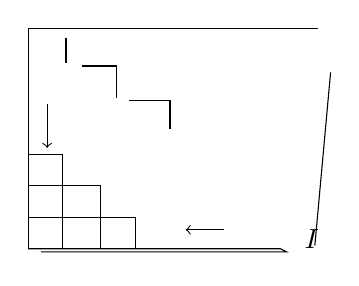
\begin{tikzpicture}[scale=.8]
\draw (0,0)--(0,3.5)--(4.6,3.5);
\draw (4.8,2.8)--(4.55,.05);
\draw (0,0)--(4,0)--(4.1,-.05)--(.2,-.05);
\draw (0,0) rectangle (.55,.5);\draw (0,.5) rectangle (.55,1);\draw (0,1) rectangle (.55,1.5);
\draw (.55,0) rectangle (1.15,.5);\draw (.55,.5) rectangle (1.15,1);\draw (1.15,0) rectangle (1.7,.5);
\draw (.6,3.35)--(.6,2.95) (.85,2.9)--(1.4,2.9)--(1.4,2.4) (1.6,2.35)--(2.25,2.35)--(2.25,1.9);
\draw[->] (.3,2.3)--(.3,1.6);\draw[->] (3.1,.3)--(2.5,.3);
\node at (4.5,.15) {$I$};
\end{tikzpicture}}

\[p\subset p'\qquad q'\subset q=m\qquad A_m/p^n A_m=B\]
\diagram{\begin{tikzcd}[ampersand replacement=\&]
A_{q,p''}\arrow[d]\&\&\\
A_{\deleted{\unsure{p}}q,p'}\arrow[d]\&A_{q',p'}\arrow[l]\arrow[d]\&\\
A_{\deleted{\unsure{p}}q,p}\&A_{q',p}\arrow[l]\&A_{q'',p}\arrow[l]
\end{tikzcd}}
\diagram{\begin{tikzcd}[ampersand replacement=\&]
\&p'\arrow[dr,no head,"\subset"]\&\\
p\arrow[ur,no head,"{\unsure{\subsetneq|\ne}}"]\arrow[dr,no head,"\subset"']\&\&q\\
\&q'\arrow[ur,no head,"\subsetneq"']\&
\end{tikzcd}}

\[\operatorname{Hom}(K_p,K_q)\]
\diagram{\begin{tikzcd}[ampersand replacement=\&]
\&p'\arrow[ur,no head,"\subsetneq"]\&p''\arrow[dr,no head,"\subset"]\&\\
p\arrow[r,no head,"\subsetneq"]\arrow[ur,no head,"\subsetneq"]\arrow[drr,no head,"\subset"']\&p'\arrow[r,no head,"\subseteq"]\&q'\arrow[r,no head,"\subsetneq"]\&q\\
\&\&q''\arrow[ur,no head,"\subsetneq"']\&q'\arrow[u,no head,"\subsetneq"']
\end{tikzcd}}
\[\underset{\longleftrightarrow}{\operatorname{Hom}(K_*,K_*)}\]
\[
A_{q,p}=(\coprod_{p'}A_{q,p'})\unsure{\amalg}(\coprod_{q'}A_{q',p})\big/
\]

$I$ ensemble ordonné, tel que

(i) deux \unsure{objets} $\deleted{\unsure{p,q}}\inserted{x,y}$ tels que $\deleted{p\leq}\,x<y$ \unsure{peuvent} être \unsure{joints} par une chaine saturée

(ii) Deux chaines saturées ont $=$ longueur

\deleted{Si $x,y$} On \unsure{suppose définis} $A_{x,y}\in\unsure{\mathcal C|\mathcal E}$ si $\left\{\begin{aligned}&\deleted{\unsure{d(x,y)}}x\leq y\\&\text{et }d(x,y)\leq1\end{aligned}\right.$

On va en construire un \deleted{\unsure{complexe, bicomplexe}} \unsure{objet} à une \unsure{``puissance''} \unsure{de $I$ indexée},
